\chapter{State of the Art}\label{chapter:SotA}
In this chapter various approaches trying to solve the placement and routing problem for QCA are reviewed. In the first part algorithms, which are able to work only with combinational circuits, are investigated under the theoretical groundwork done in chapter \ref{chapter:Preliminaries}. First the use both algorithms determining \textit{optimal} and those who determine \textit{scalable} solutions are explained. In the second part ideas and challenges of sequential placement and routing algorithms are investigated.

\section{Combinational P\&R Algorithms}
In order to understand optimal solutions for placement and routing, it has to be reviewed from section \ref{sec:PR} that this problem is $\mathcal{NP}$-hard. Here the complexity class $\mathcal{NP}$ (nondeterministic polynomial time) describes a set of decision problems, where problem instances with a formula, that can be evaluated to true, have a proof, that can be verified in polynomial time by a deterministic Turing machine. The existence of these problems lead to several ideas on solving them, one of these being \textit{Satisfiability Modulo Theories} (SMT). The \textit{satisfiability problem} can be formulated as the question if there exists a model evaluating the first-order formula over some theories to true. The consequent solving instance for propositional logic is a \textit{Boolean Satisfiability Solver} (SAT), with proposition being Boolean equations, that have to be proven true. With this basic instance two different solving strategies were proposed. The first strategy is called \textit{Eager SMT-solving} and is used for uninterpreted functions or bit-vectors, which can be derived to propositional logic. Therefore the first step implies the transformation of theory constraints into \textit{equisatisfiable} propositional logic. These problem insances are then passed to SAT solvers, checking for satisfiability. Due to the equisatisfiability, a solution for the original problem can be derived from the solution of the propositional logic. The second approach \textit{lazy SMT-solving} refers to the assisting use of \textit{theory solvers} and is depicted in figure \ref{fig:SMT_solving}. In the first step the first-order problem with formula $\varphi$ is transformed to a \textit{Boolean abstraction} $\varphi'$ mapping the concrete problem to an abstract problem under a set of finite Boolean predicates \cite{boolean_abstraction}. The abstraction is then passed to the SAT-solver, which again computes solutions and gives them to a set of theory solvers. They again check if the Boolean predicates hold true thus if they are consistent in the provided solution. If so the abstraction is satisfiability and the theory solver instance returns SAT. Otherwise UNSAT with an explanation is passed back to the SAT-solver so that the abstraction can be improved. If the abstraction is found to be unsatisfied the problem is said to be unsatisfiable.
\cite{SMT}

\begin{figure}
	\centering
	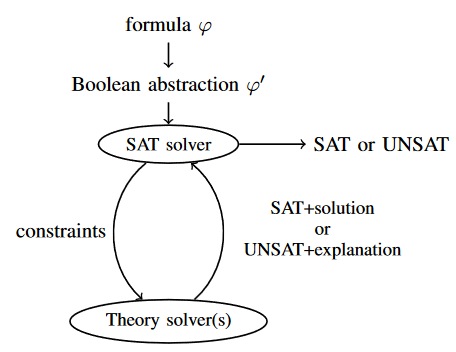
\includegraphics[scale=0.8]{SMT_solving}
	\caption{Lazy SMT-solving  process \cite{SMT}}\label{fig:SMT_solving}
\end{figure}

With this knowledge optimal placement and routing algorithms can be discussed. Two approaches from \cite{Walter} are reviewed for this. The first algorithm "Exact Placement and Routing" finds a valid placement, routing and clocking, also described as $(p, r, c)$, given an empty layout $L$ and a logic network $N$. In order to find an optimal solution, the minimum layout size $w \times h$
has to be determined for which the constraints of $(p, c, r)$ hold true. Therefore all possible sizes of layouts are encoded and passed to a SAT-solver iteratively and the first layout for which the solver returns true is the minimum or rather optimal solution. The experimental results show that the determined layouts of the algorithm are many times smaller than the compared state of the art CITE. But due to the complexity of the algorithm utilizing satisfiability solvers, the algorithm times out for quite small circuits already, making it insufficient for the manufacturing of commercial QCA circuits.\\
In the book \cite{Walter} another exact P\&R algorithm is proposed. The idea is to create a \textit{one-pass synthesis}, which combines logic synthesis and physical design in a single run. Therefore this algorithm has to tackle two $\mathcal{NP}$-hard problems relying again on the power of satisfiability solvers. This particular algorithm uses eager SMT-solving. The idea is to eliminate some shortcomings of the two-step synthesis derived from CMOS. This includes treating wires as gates since the costs are equal in QCA and including data synchronization, which is dependent on the tiles passed. In this manner a SAT problem can be formed and passed to a SAT-solver. The instances are now created only passing a empty layout $L$ of size $w \times h$. Even though this algorithm is able to find \textit{truly minimal} solution since the non-optimal logic networks are eliminated, the experimental results show the same problems as in the exact P\&R approach. This means that the high complexity of the satisfiability solver leads to a time-out of the algorithms for circuits with a gate size $|N| \geq 30$.\\
These results lead to the usage of scalable placement and routing algorithms. These approaches trade optimality of the circuit, like layout size for computing time. This makes them scalable in the time domain and therefore applicable for the manufacturing of commercial QCA circuits. All algorithms reviewed in the following are based on the original VLIS process, meaning they treat logic synthesis and physical design as their own problem.\\
Starting at the logic synthesis many works present a preprocessing of logic networks to make them suitable to translate them into gate level representations. There are several steps which are widely used to modify logic networks. The first of them is the node duplication or rather dummy node insertion. The idea of this process is to minimize wire-crossings, which we have analyzed to be very costly in QCA. Also the fanouts of the nodes are reduced, leading to a reduction of the place and rout complexity. One simple algorithm for this is to visit every node iteratively from the primary outputs to the primary inputs. If the current node hasn't been visited its marked as visited and if a already marked node is visited it is duplicated. But this means that not only one node is duplicated but also all the nodes included in te sub tree rooted by it \cite{QCA-LG}. From this simple example we can already suggest that the insertion of dummy nodes can lead to uncontrollable growth of the logic network. Other algorithms which are not that dedicated, don't have such a high overhead in dummy nodes but therefore can't eliminate all wire crossings making it necessary to include nodes for crossings, so called \textit{crossing edge insertions} \cite{node_duplication}. Another preprocessing steps including the insertion of so called \textit{buffer nodes} is the synchronization- Since the global timing constraint requires two paths leading to the same node to pass the same amount of tiles, this step makes sure that every two paths leading to a node include the same amount of gates. A buffer node therefore indicates that wires in QCA have to be viewed as gates as well. Also due to the insertion of buffers different partitions of a logic network can be generated \cite{dummy_and_buffer_nodes}. Some approaches lead to even higher insertion of nodes indicating wasted area. This arises from the idea of a complete ternary logic network representation of a QCA circuit, since the gates are based on majority functions GRAPH . When extra area is produced due to the insertion of nodes, also wire lengths can be increased. For gates with two or three inputs, this means that if the longest wire has to be split into more than one clock zone, also the shortest wire has to be split into the same amount of clock zones in order to preserve the signal synchronization \cite{QCA-LG}. Another big problem of these algorithms is the requirement of cell-based clocking, which we have already showed to be insufficient. Even though there also exist algorithms using tile-based clocking they are limited by the general drawbacks of preprocessing \cite{trindade2016placement} leading to exploding logic networks and even use greedy placement and routing algorithms limiting the approach to small and simple reconvergent patterns \cite{greedy_tile}.\\

All these reasons lead to the proposal of \textit{ortho}, an algorithm implementing a scalable placement, routing and clocking without preprocessing steps \cite{ortho}. Since this algorithms forms the base of this work, the algorithm is explained detailed in the following.\\
First of all, a proper representation of the logic network is needed. Therefore in some works already the idea of an orthogonal embedding, have been proposed \cite{dummy_and_buffer_nodes}. This means that the logic network is mapped onto a two-dimensional grid, so it can be seen as an assignment of the tuple $(p, r)$. For ortho this is done by \text{orthogonal graph drawing} (OGD), which is described in \cite{OGD}.

\begin{definition}[Orthogonal Graph Drawing]
	An OGD maps a graph $G = (V, E)$ onto a plane grid with size $w \times h$. The mapping assigns vertices $v \in V$ with coordinates $(x, y)$ to grid points, with $1 \leq x < w$ and $1 \leq y < h$. Edges $e \in E$ are assigned to paths in the grid, so they consist only from horizontal and vertical segments. The paths are non-overlapping, meaning that they are not allowed to cross any vertices.
\end{definition}

Figure \ref{fig:OGD_example} shows an example OGD. The dots in the graph represent vertices and are connected via straight line paths. Therefore the graph is drawn orthogonally.

\begin{figure}
	\centering
	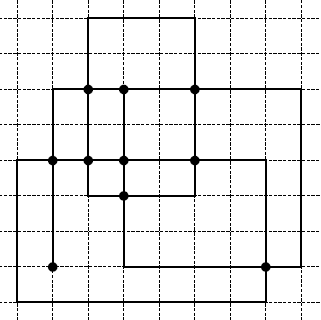
\includegraphics[scale=0.7]{OGD}
	\caption{Example OGD drawing}\label{fig:OGD_example}
\end{figure}

Nonetheless an OGD also only respects the placement and routing, leaving the clocking to be addressed. The problem of insufficient clocking out of an OGD representation can be showed from the example in \cite{Walter}. Figure \ref{fig:OGD_timing} shows, that for a given OGD (\ref{subfig:OGD_sync_b}) there has to be no clocking which can resolve the timing constraints (\ref{subfig:OGD_sync_c}). It stands out that for the down right corner no clocking zone can be found that is satisfies the local synchronization constraint but also the global synchronization constraint is violated. Since the clocking or rather signal synchronization was a main task of the preprocessing now some other solution has to be found.

\begin{figure}
	\newcommand*{\xMin}{0}%
	\newcommand*{\xMax}{3}%
	\newcommand*{\xMaxc}{2}%
	\newcommand*{\yMin}{0}%
	\newcommand*{\yMax}{3}%
	\newcommand*{\yMaxc}{2}%
	\centering
	\subfigure[Partial representation of a logic network]
	{
		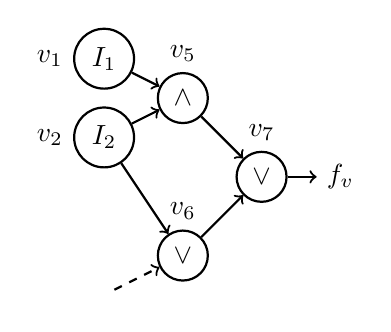
\begin{tikzpicture}[node distance={2cm and 2cm}, thick, scale=0.5, main/.style = {draw, circle}] 
			\node[main] (1) at (0,0) [label=west:$v_1$]{$I_1$}; 
			\node[main] (2) at (0,-2)[label=west:$v_2$] {$I_2$};
			\node (3) at (0,-4) {};
			\node (4) at (0,-6) {};
			
			\node[main] (5) at (2,-1)[label=north:$v_5$]{$\wedge$}; 
			\node[main] (6) at (2,-5)[label=north:$v_6$]{$\vee$};
			
			\node[main] (7) at (4,-3)[label=north:$v_7$]{$\vee$};
			
			\node (f) at (6,-3) {$f_v$};
			
			
			\draw[->] (1) -- (5);
			\draw[->] (2) -- (5);
			\draw[->] (2) -- (6);
			\draw[dashed, ->] (4) -- (6);
			\draw[->] (5) -- (7);
			\draw[->] (6) -- (7);
			\draw[->] (7) -- (f);
			
		\end{tikzpicture} 
	}
	\subfigure[OGD representation of the logic network]
	{
		\centering
		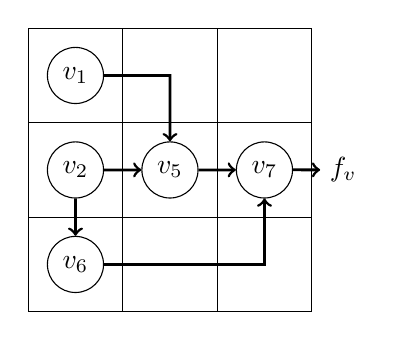
\begin{tikzpicture}[scale=1.2, main/.style = {draw, circle, fill=white}]
			
			\draw[fill=white]  (0, 2) -- (1, 2) -- (1,1) -- (0,1) -- cycle;
			\draw[fill=white]  (1, 2) -- (2, 2) -- (2,1) -- (1,1) -- cycle;
			\draw[fill=white]  (2, 2) -- (3, 2) -- (3,1) -- (2,1) -- cycle;
			
			
			\draw[fill=white]  (0, 3) -- (1, 3) -- (1,2) -- (0,2) -- cycle;
			\draw[fill=white]  (1, 3) -- (2, 3) -- (2,2) -- (1,2) -- cycle;
			\draw[fill=white]  (2, 3) -- (3, 3) -- (3,2) -- (2,2) -- cycle;
		
			
			\draw[fill=white]  (0, 4) -- (1, 4) -- (1,3) -- (0,3) -- cycle;
			\draw[fill=white]  (1, 4) -- (2, 4) -- (2,3) -- (1,3) -- cycle;
			\draw[fill=white]  (2, 4) -- (3, 4) -- (3,3) -- (2,3) -- cycle;
			
			
			\node[main] (1) at (0.5, 3.5) {$v_1$}; 
			\node[main] (2) at (0.5, 2.5) {$v_2$};

			\node[main] (5) at (1.5,2.5){$v_5$}; 
			\node[main] (6) at (0.5,1.5){$v_6$};
			
			\node[main] (7) at (2.5,2.5){$v_7$};
			
			\node [right of = 7] (f) {$f_v$};
			
			
			\draw[->, line width = 1pt] (1) -- (1.5, 3.5) -- (5);
			\draw[->, line width = 1pt] (2) -- (5);
			\draw[->, line width = 1pt] (2) -- (6);
			\draw[->, line width = 1pt] (5) -- (7);
			\draw[->, line width = 1pt] (6) -- (2.5, 1.5) -- (7);
			\draw[->, line width = 1pt] (7) -- (f);

			
			
		\end{tikzpicture}
		\label{subfig:OGD_sync_b}
	}
	\subfigure[No sufficient clocking for this OGD can be examined]
	{
		\centering
		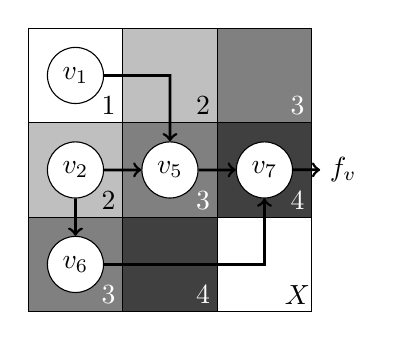
\begin{tikzpicture}[scale=1.2, main/.style = {draw, circle, fill=white}]
			
			\draw[fill=gray]  (0, 2) -- (1, 2) -- (1,1) -- (0,1) -- cycle;
			\draw[fill=darkgray]  (1, 2) -- (2, 2) -- (2,1) -- (1,1) -- cycle;
			\draw[fill=white]  (2, 2) -- (3, 2) -- (3,1) -- (2,1) -- cycle;
			
			
			\draw[fill=lightgray]  (0, 3) -- (1, 3) -- (1,2) -- (0,2) -- cycle;
			\draw[fill=gray]  (1, 3) -- (2, 3) -- (2,2) -- (1,2) -- cycle;
			\draw[fill=darkgray]  (2, 3) -- (3, 3) -- (3,2) -- (2,2) -- cycle;
			
			
			\draw[fill=white]  (0, 4) -- (1, 4) -- (1,3) -- (0,3) -- cycle;
			\draw[fill=lightgray]  (1, 4) -- (2, 4) -- (2,3) -- (1,3) -- cycle;
			\draw[fill=gray]  (2, 4) -- (3, 4) -- (3,3) -- (2,3) -- cycle;
			
			\node[text=white] (A1) at (0.85,1.18) {$3$};
			\node[text=white] (A1) at (1.85,1.18) {$4$};
			\node[text=black] (A1) at (2.85,1.18) {$X$};
			
			
			\node[text=black] (A1) at (0.85,2.18) {$2$};
			\node[text=white] (A1) at (1.85,2.18) {$3$};
			\node[text=white] (A1) at (2.85,2.18) {$4$};
			
			
			\node[text=black] (A1) at (0.85,3.18) {$1$};
			\node[text=black] (A1) at (1.85,3.18) {$2$};
			\node[text=white] (A1) at (2.85,3.18) {$3$};
			
			\node[main] (1) at (0.5, 3.5) {$v_1$}; 
			\node[main] (2) at (0.5, 2.5) {$v_2$};
			
			\node[main] (5) at (1.5,2.5){$v_5$}; 
			\node[main] (6) at (0.5,1.5){$v_6$};
			
			\node[main] (7) at (2.5,2.5){$v_7$};
			
			\node [right of = 7] (f) {$f_v$};
			
			
			\draw[->, line width = 1pt] (1) -- (1.5, 3.5) -- (5);
			\draw[->, line width = 1pt] (2) -- (5);
			\draw[->, line width = 1pt] (2) -- (6);
			\draw[->, line width = 1pt] (5) -- (7);
			\draw[->, line width = 1pt] (6) -- (2.5, 1.5) -- (7);
			\draw[->, line width = 1pt] (7) -- (f);
			
			
			
		\end{tikzpicture}
		\label{subfig:OGD_sync_c}
	}
	
	\caption{Insufficient timing constraints of a OGD representation \cite{Walter}}\label{fig:OGD_timing}
\end{figure}

The idea used for the ortho algorithm comes from an extension to OGDs , which allows to determine a special OGD from a logic network in polynomial time being the constraint needed for a scalable approach. The base used here is formed by Therese Biedl \cite{biedl1998better}, who proposes a OGD with an additional edge coloring. Although the effectiveness and complexity bounds in her work were proven on the restriction of \textit{undirected 3-graphs} and as we already examined from the precious chapter a logic network is neither containing only nodes of most degree 3 nor undirected. To overcome the fist restriction, a custom logic network can be created by assigning own nodes for fanouts and inverters. This way the maximum node degree gets decreased to three, while the expressiveness of the logic network representation is maintained. The second restriction can be overcome by a custom coloring built on the original approach, which also serves as direction assignment. Given a logic network converted to a 3-graph, the coloring in form of edge directions $d : \Delta \rightarrow \{east, south\}$ is assigned. The coloring can be understood as relative position arrangement. If an edge $(v_i, v_j)$ is colored $east$, means that the vertex $v_j$ is positioned east of $v_i$, so that $x_j > x_i$. The color $south$ for an edge $(v_i, v_j)$ assigns $v_j$ a relative position of $v_i$, so that $v_j$ is south of $v_i$ or $y_j > y_i$. In order to color a graph with only these two colors the following \textit{assignment constraints} must hold true:
\begin{enumerate}
	\item All \textbf{incoming} edge of a vertex has to be painted with the \textbf{same} color.
	\item All \textbf{outgoing} edges of a vertex have to be painted with \textbf{opposite} colors.
\end{enumerate}

The relative position assignment under the proposed constraints can be seen at an arbitrary example in figure \ref{fig:OGD_color}. In the example for outgoing edges (figure \ref{subfig:OGD_color_out}), it is clear that the assignment constraint makes sure that two outgoing edges of the same vertex are routed without conflict. Due to the definition of the colors, the layout is increased in x-direction for an east-coloring and analogously extended in the y-Direction for a south-coloring. Figure \ref{subfig:OGD_color_in} depicts the assignment constraint for the incoming edges of one vertex. Since this implies only one color, also the layout only is extended in one direction, here in x-direction due to the east-coloring. The clocking used in the example is 2DD-Wave, because it also supports only signal flow in the directions $east$ and $south$. This means that the local synchronization constraint is always true if we use this scheme. But due to its uniformity the scheme also maintains the global synchronization constraint for vertices placed after the proposed direction assignment. This is why ortho utilizes the 2DD-Wave scheme. However, there exist logic networks for which no coloring holding the constraints can be found. Figure \ref{fig:Coloring_conflict} shows such a coloring conflict. For the edge with a "$X$", no direction can be assigned for which the formulated constraints hold true. So an auxiliary node is introduced resolving the conflict.\\
The ortho algorithm can be described as follows. 

Figure !! depicts the pseudo code for it.
The example depicted in figure !! shows the $(p, r, c)$ of a 2:1 mux.

\begin{figure}
	\centering
	\subfigure[Color assignment of incoming signals]
	{
		\centering
		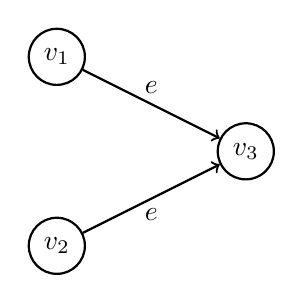
\begin{tikzpicture}[node distance={2cm and 2cm}, thick, scale=1.2, main/.style = {draw, circle}] 
			\node[main] (1) at (0,0) {$v_1$}; 
			\node[main] (2) at (0,-2){$v_2$};
			
			\node[main] (3) at (2,-1){$v_3$}; 
			
			\draw[->, above] (1) -- (3) node [midway] {$e$};
			\draw[->, below] (2) -- (3) node [midway] {$e$};
			
		\end{tikzpicture} 
		\label{subfig:OGD_color_out}
	}
	\subfigure[Color assignment of outgoing signals]
	{
		\centering
		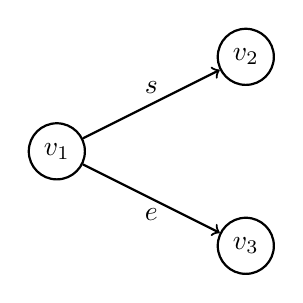
\begin{tikzpicture}[node distance={2cm and 2cm}, thick, scale=1.2, main/.style = {draw, circle}] 
			\node[main] (1) at (0,-1) {$v_1$}; 
			\node[main] (2) at (2,0){$v_2$};
	
			\node[main] (3) at (2,-2){$v_3$}; 
			
			\draw[->, above] (1) -- (2) node [midway] {$s$};
			\draw[->, below] (1) -- (3) node [midway] {$e$};
			
		\end{tikzpicture} 
		\label{subfig:OGD_color_in}
	}
	
	\caption{Relative positions of an OGD graph with correct color assinment}\label{fig:OGD_color}
\end{figure}

%\begin{figure}
%	\centering
%	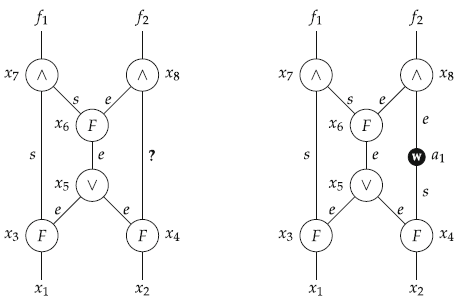
\includegraphics[scale=0.7]{Coloring_conflict}
%	\caption{Solution for a coloring conflict}\label{fig:Coloring_conflict}
%\end{figure}

\algnewcommand\algorithmicforeach{\textbf{for each}}
\algdef{S}[FOR]{ForEach}[1]{\algorithmicforeach\ #1\ \algorithmicdo}
\begin{algorithm}[H]
	\hspace*{\algorithmicindent} \textbf{Input:} Logic network $N$ \\
	\hspace*{\algorithmicindent} \textbf{Input:} Clock number $clk$\\
	\hspace*{\algorithmicindent} \textbf{Output:} Gate level layout $L$
	\begin{algorithmic}[1]
		\State Convert $N$ to a 3-graph by substitution
		\State $L \leftarrow$ empty 2DDWave-clocked layout of size $w = 0 \times (h = 0)$
		\State Generate direction assignment $d : \Delta \rightarrow \{east, south\}$ and subdivide signals if necessary
		\State Compute topological ordering $v_1, . . . , v_i \in N$
		\State Extend $L$ by one column and reserve it for primary inputs
		\ForEach {primary input $v_1, ..., v_l \in N $}
		\State Extend $L$ by one row
		\State Place v at position $(0, h - 1)$
		\EndFor
		\ForEach {primary input $v_1, ..., v_l \in N $}
		\State Extend $L$ by one column and one row
		\State Wire the primary input to position $(w - 1, h - 1)$ 
		\EndFor
		\ForEach {vertex $v_l+1, ..., v_i \in N $ with at most two incoming signals $\sigma_1, \sigma_2$}
		\If{$d(\sigma_1) = d(\sigma_2) = east$}
		\State Extend $L$ by one column
		\State $h_p \leftarrow$ max. vertical position of v's predecessors
		\State Place v at position $(w - 1, h_p)$
		\Else { signals are labeled $south$}
		\State Extend $L$ by one row
		\State $w_p \leftarrow$ max. horizontal position of v's predecessors
		\State Place v at position $(w _p, y - 1)$
		\EndIf
		\State Extend $L$ by one column and one row
		\State Wire the primary input to position $(w - 1, h - 1)$ 
		\EndFor
		\State Draw orthogonal wire segments to connect v with its predecessor(s) accordingly
		\State Connect the primary outputs to the respective borders
		\Return $L$
	\end{algorithmic}
	\caption{Ortho algorithm}\label{alg:ortho}
\end{algorithm}

\section{Sequential P\&R Algorithms}
Present the ideas in papers for QCA standard cell placement and routing. \\
Point out why they are not actionable: Reasons like clocking or cells aren't producible, no automated algorithms